\documentclass[paper=a4,oneside,abstract,DIV=19,parskip=half]{scrartcl}
\usepackage[utf8]{inputenc} %+Umlaute
\usepackage{csquotes}
\usepackage[ngerman]{babel}
\usepackage[backend=biber,
date=long,
style=iso-numeric,
autolang=other,
%bibencoding=UTF8
]{biblatex}
\addbibresource{dtlab-verzoeg.bib}
% Literaturverzeichnis mit Nummern in Klammern wie [3]
\DeclareFieldFormat{labelnumberwidth}{[#1]}
\setcounter{biburllcpenalty}{7000}
\setcounter{biburlucpenalty}{8000}
\usepackage{hyperref}

\usepackage{graphicx}
\usepackage{siunitx}
\sisetup{separate-uncertainty,locale=DE}

\title{Verzögerungszeit eines 74HC00 NAND Gatters}
\subject{Messbericht}
\titlehead{}
\author{Günther Mößmer und Friedrich Beckmann}
\date{Messung: 4. April 2024 / Bericht: 11. April 2024}

\begin{document}
\shorthandoff{"}
\maketitle
\begin{abstract}
\noindent Wir haben die Verzögerungszeit einer Inverterkette aus vier NAND Gattern eines 74HC00 Bausteins bei \SI{5}{\V} und \SI{2}{\V}  Betriebsspannung gemessen und mit den Werten aus dem Datenblatt verglichen. Die gemessene Verzögerungszeit von \qty{39,8(10)}{\ns} bei \SI{5}{\V} und \qty{186(5)}{\ns} bei \SI{2}{\V}  liegt im Rahmen der zu erwartenden Werte aus dem Datenblatt.
\end{abstract}

\section{Messung der Verzögerungszeit}
Die Verzögerungszeit wird zwischen Eingang und Ausgang der Schaltung bei 50 Prozent des Highpegels gemessen. Der Highpegel am Eingang wird auf die Betriebsspannung gesetzt. 
\begin{figure}[!htb]
\begin{center}
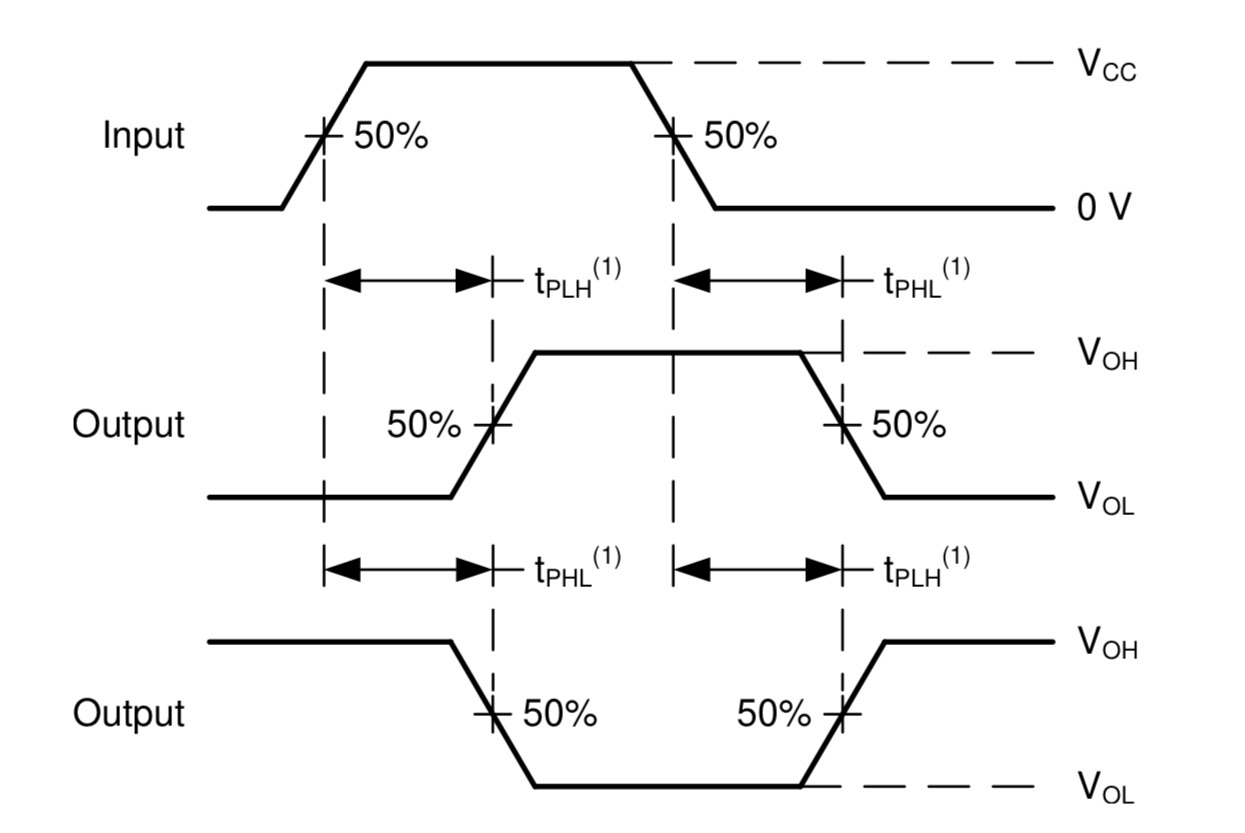
\includegraphics[width=0.5\textwidth]{messprinzip}
\end{center}
\caption{Definition der Verzögerungszeiten aus dem Datenblatt des IC \cite[Figure 7-2]{ti74hc00}}
\label{fig:messprinzip}
\end{figure}
In Abbildung \ref{fig:messprinzip} aus dem Datenblatt ist dargestellt wie die Verzögerungszeiten $t_{\textrm{pLH}}$ und $t_{\textrm{pHL}}$ definiert sind \cite[Figure 7-2]{ti74hc00}.

\section{Messaufbau}

Wir haben die vier NAND Gatter des 74HC00 Bausteins wie im Schaltplan in Abbildung \ref{fig:schaltplan} dargestellt als Inverterkette anhand des vorliegenden Datenblatts verschaltet \cite{ti74hc00}. Der Anschluss VCC an Pin 14 des IC wurde mit dem Labornetzteil mit \SI{+5}{\V} (später \SI{2}{\V}) versorgt. Die Masse des Labornetzteils ist mit Pin 7 (GND) des IC verbunden.

\begin{figure}[!htb]
\begin{center}
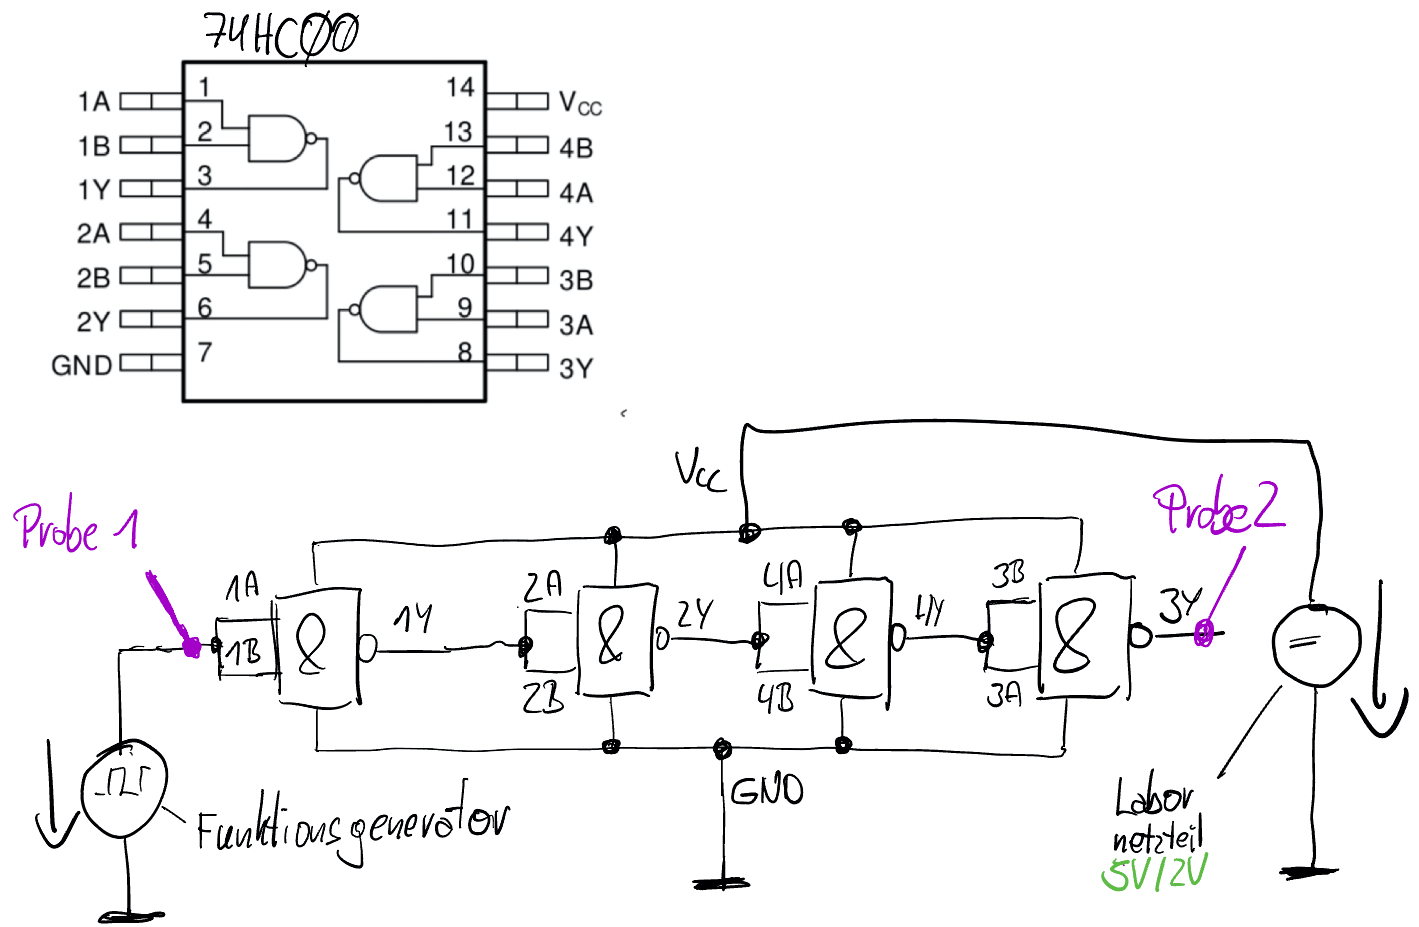
\includegraphics[width=0.8\textwidth]{schaltplan}
\end{center}
\caption{Schaltplan der Inverterkette aus 4 NAND Gattern mit Probes und Funktionsgenerator}
\label{fig:schaltplan}
\end{figure}

\begin{figure}[!htb]
\begin{center}
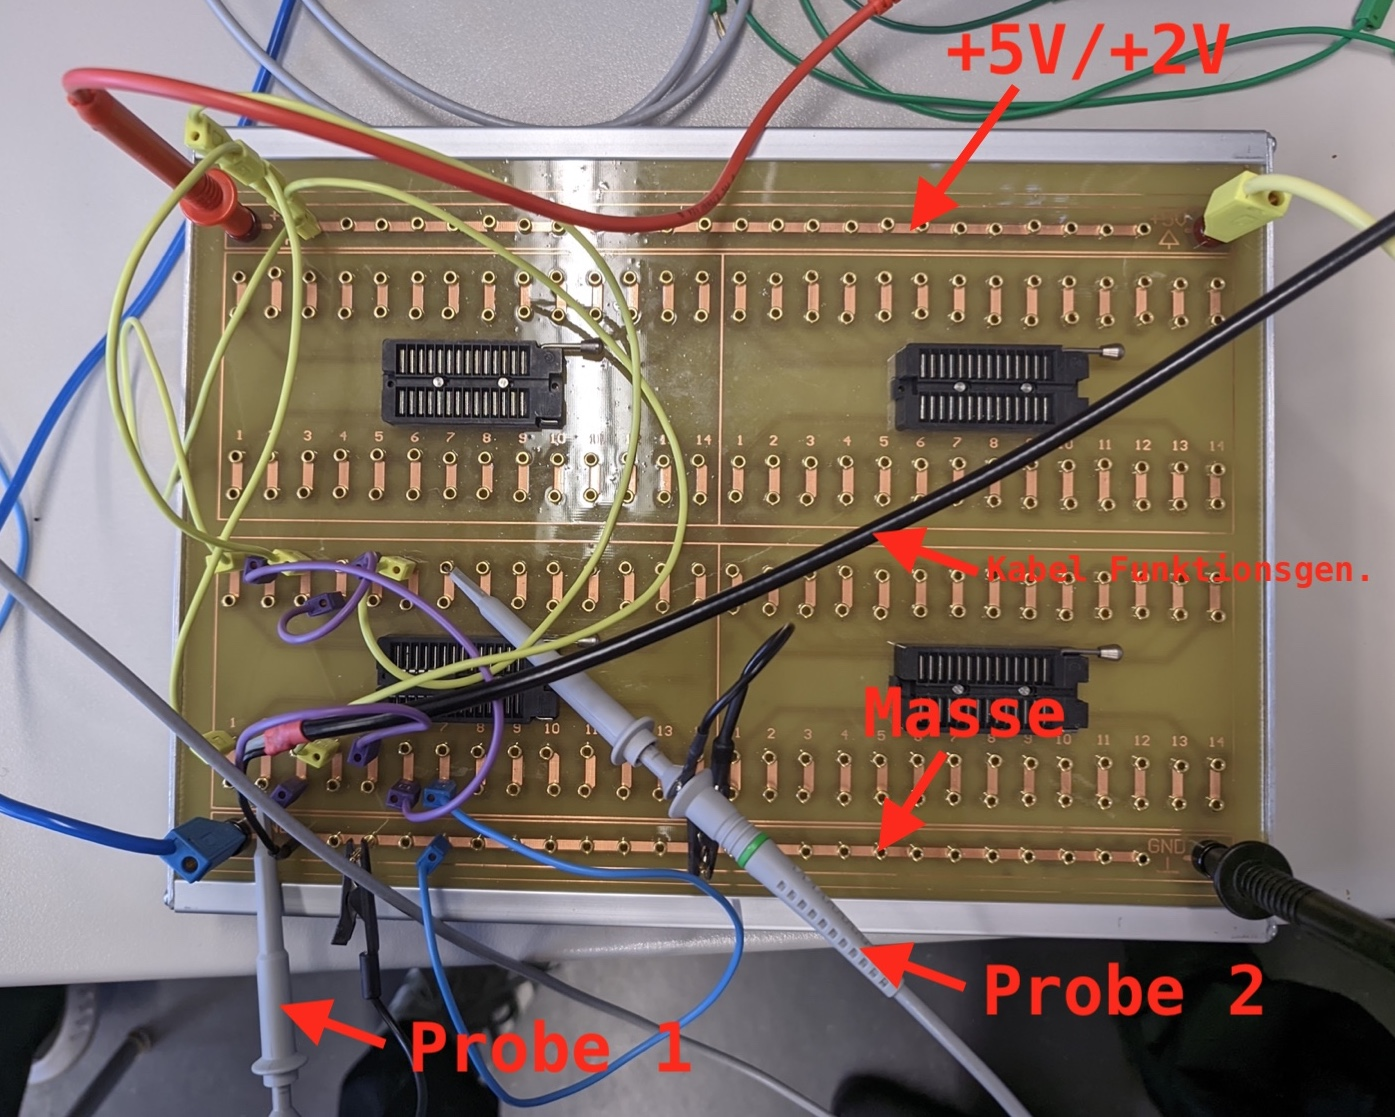
\includegraphics[width=0.8\textwidth]{board}
\end{center}
\caption{Foto des ZIF Boards mit dem 74HC00 IC, den Kabeln und den Probes}
\label{fig:zifboard}
\end{figure}

Der Funktionsgenerator hat einen BNC Anschluss. Wir haben ein Kabel mit einem BNC Stecker an einem Ende zum Anschluss an den Funktionsgenerator und zwei \SI{2}{\mm} Bananensteckern am anderen Ende für den Anschluss an das Board verwendet. Der Massestecker (schwarz) des Kabels ist in die Masseleiste des Boards eingesteckt. Der Stecker mit dem Signal vom Funktionsgenerator (rot) ist in die Buchse von Pin 2 (1B) des IC gesteckt. 

Am Oszilloskop wird der Kanal 1 mit einer Probe (gelb) an den Eingang 1B (Pin 2) des IC angeschlossen. Wir haben dazu einen \SI{2}{\mm} Messingstecker verwendet und die Probe dort mit dem Klemmhaken befestigt. Kanal~2 ist über die grüne Probe mit Pin 8 (3Y) des IC verbunden. Die Masseklemmen der Probes sind mit einem \SI{2}{\mm} Messingstecker mit der Masse des Boards verbunden. Abbildung \ref{fig:zifboard} zeigt ein Foto des ZIF Boards mit dem 74HC00 IC, den Kabeln und den Probes. Unten ist die Masseleitung zu sehen. Die Chipmarkierung des IC haben wir als \glqq UTC RKTV U74HC00L 01\grqq\,  abgelesen. Es handelt sich wahrscheinlich nicht um einen Baustein von Texas Instruments wie der im Datenblatt beschriebene IC, sondern um ein Produkt von UTC.

Vor der Messung der Verzögerungszeit haben wir statisch die Funktion mit dem Multimeter überprüft. Ohne den Funktionsgenerator haben wir die Betriebsspannung auf \SI{5}{\V} (gemessen: \SI{4,983}{\V}) eingestellt und den Eingang 1B des IC mit einem Kabel mit Masse verbunden. Dann haben wir mit dem Multimeter die Spannungen an allen Pins gemessen und so statisch die Funktion der Inverterkette überprüft.

\newpage
\section{Messung mit 5 Volt Betriebsspannung}

Wir haben die Betriebsspannung am Labornetzteil auf \SI{5}{\V} eingestellt. Mit dem Multimeter haben wir an Pin 14 (VCC) des IC \SI{4,987}{\V} gemessen. Den Funktionsgenerator haben wir auf eine Frequenz von \SI{1}{\MHz}, einen Highpegel von \SI{5}{\V} und einen Lowpegel von \SI{0}{\V} eingestellt.

\begin{figure}[!htb]
\begin{center}
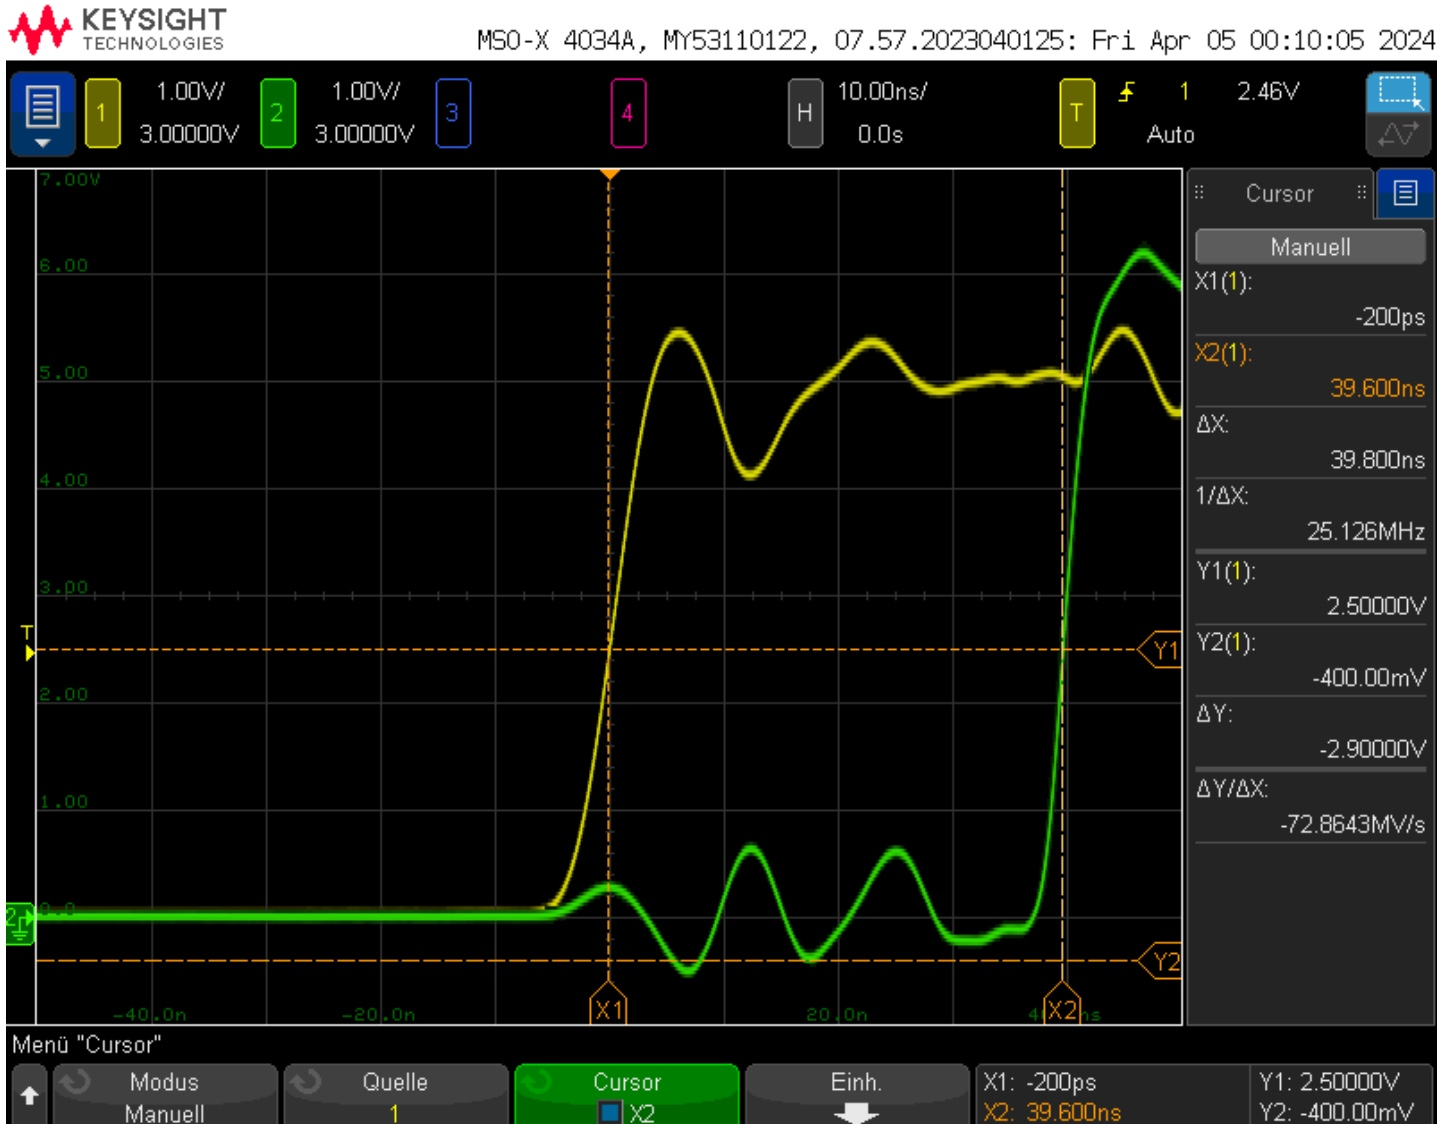
\includegraphics[width=0.99\textwidth]{messung5v}
\end{center}
\caption{Screenshot vom Oszilloskop bei der Messung der Verzögerungszeit bei \SI{5}{\V}}
\label{fig:mess5v}
\end{figure}

Abbildung \ref{fig:mess5v} zeigt einen Screenshot des Oszilloskops mit dem zeitlichen Verlauf der Signale an Kanal 1 (gelb, 1B, Pin 2) und an Kanal 2 (grün, 3Y, Pin 8). Kanal 1 (gelb) zeigt also das Signal am Eingang der Inverterkette und Kanal 2 (grün) das Signal am Ausgang der Inverterkette. Die Kanäle 1 und 2 sind beide auf \SI{1}{\V\per Div} und einen Offset von \SI{3}{\V} eingestellt. Das Scope triggert auf Kanal 1 (Eingangssignal) auf eine steigende Flanke. Der Triggerlevel ist auf \SI{2,46}{\V} eingestellt um den Triggerzeitpunkt ein einem möglichst steilen Signaldurchgang durch den Triggerlevel zu haben. Man sieht, dass das Signal an Kanal~2 (Ausgang) zeitlich versetzt dem Signal an Kanal 1 (Eingang) folgt. Die Verzögerungszeit wird bei einer steigenden Flanke am Ausgang bei 50 Prozent des Highpegels gemessen. Wir haben den Cursor Y1 deshalb auf \SI{2,5}{\V} (=50 Prozent Highpegel) eingestellt und den Cursor X1 auf den Schnittpunkt von Cursor Y1 und der steigenden Flanke vom Eingangssignal auf Kanal 1 gelegt. Cursor X2 ist auf den Schnittpunkt des Ausgangssignals auf Kanal~2 mit Y1 gelegt. Die Zeitdifferenz der Cursor X1 und X2 entspricht deshalb der Verzögerungszeit bei einer steigenden Flanke am Ausgang $t_{\textrm{pLH}}$. In Abbildung \ref{fig:mess5v} kann man rechts die Position von Cursor X1 (\SI{-200}{\ps}) und X2 (\SI{39,600}{\ns}) und die Differenz $\Delta x$ von \SI{39,800}{\ns} ablesen. 

Die horizontale Ablenkung ist auf \SI{10}{\ns\per Div} eingestellt. Wir können den Cursor mit etwa $\pm$\SI{0,5}{\ns} (=1/20 Div) Genauigkeit einstellen. Der Fehler für die Differenz der Zeiten beträgt demnach $\pm$\SI{1}{\ns}. Die gemessene Verzögerungszeit durch die Inverterkette beträgt also \SI{39,8(10)}{\ns}.

Im Datenblatt ist für eine Temperatur von \SI{25}{\celsius} eine Verzögerungszeit bei \SI{4,5}{\V} Betriebsspannung von typisch \SI{9}{\ns} und maximal \SI{18}{\ns} angegeben \cite[Kapitel 6.7 Switching Characteristics - Commercial]{ti74hc00}. Da in der Inverterkette vier Inverter hintereinander geschaltet sind ist die zu erwartende typische Verzögerungszeit viermal \SI{9}{\ns}~=~\SI{36}{\ns}. Die maximale Verzögerungszeit beträgt \SI{72}{\ns}. Damit liegt die gemessene Verzögerungszeit von \SI{39,8(10)}{\ns} im Bereich der erwarteten Verzögerungszeit.

\section{Messung mit 2 Volt Betriebsspannung}

Für die Messung der Verzögerungszeit wurde die Betriebsspannung auf \SI{2}{\V} am Labornetzteil eingestellt. Eine Messung mit dem Multimeter an Pin 14 (VCC) ergab eine Spannung von \SI{1,982}{\V}. Den Funktionsgenerator haben wir auf eine Frequenz von \SI{1}{\MHz}, einen Highpegel von \SI{2}{\V} und einen Lowpegel von \SI{0}{\V} eingestellt.

\begin{figure}[!htb]
\begin{center}
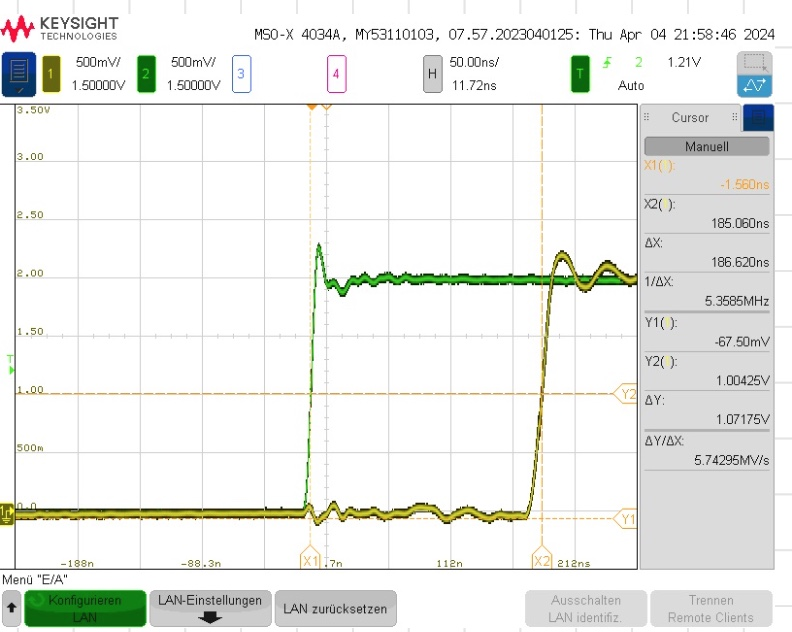
\includegraphics[width=0.99\textwidth]{messung2v}
\end{center}
\caption{Screenshot vom Oszilloskop bei der Messung der Verzögerungszeit bei \SI{2}{\V}}
\label{fig:mess2v}
\end{figure}

In Abbildung \ref{fig:mess2v} ist der Screenshot des Oszilloskops für die Messung der Verzögerungszeit bei \SI{2}{\V} Betriebs\-spannung dargestellt. Man sieht den zeitlichen Verlauf des Eingangssignals an Kanal 2 (grün) und des Ausgangssignals an Kanal 1 (gelb). Der Cursor X1 wurde an den Punkt gesetzt, bei dem die steigende Flanke den Wert von 50 Prozent des Highpegels (hier: \SI{1}{\V}) erreicht. Der Cursor X2 ist an dem Punkt, an dem die Flanke am Ausgang \SI{1}{\V} erreicht. In Abbildung \ref{fig:mess2v} kann rechts die Zeitdifferenz der Cursor $\Delta x$ von \SI{186,620}{\ns} abgelesen werden.

Die Zeitablenkung ist auf \SI{50}{\ns\per Div} eingestellt. Wir können die Cursor in etwa auf $\pm$\SI{2,5}{\ns} genau auf dem Bildschirm positionieren. Damit ergibt sich eine Genauigkeit bei der Differenz von $\pm$\SI{5}{\ns}. Die gemessene Verzögerungszeit beträgt deshalb \SI{186(5)}{\ns}.

Im Datenblatt ist für eine Temperatur von \SI{25}{\celsius} eine Verzögerungszeit bei \SI{2}{\V} von typisch \SI{45}{\ns} und maximal \SI{90}{\ns} angegeben \cite[Kapitel 6.7 Switching Characteristics - Commercial]{ti74hc00}. Die zu erwartende Verzögerungszeit für die Inverterkette liegt deshalb im Bereich von \qtyrange{180}{360}{\ns}. Die gemessene Verzögerungszeit von \SI{186(5)}{\ns} liegt im erwarteten Bereich.

\section{Verwendete Geräte}

In Tabelle \ref{tab:messg} sind die verwendeten Messgeräte aufgeführt.

\begin{table}[!htb]
\caption{Liste der verwendeten Messgeräte}
\label{tab:messg}
\centering
\begin{tabular}{lll}
Gerät & Modell & Hersteller \\\hline
Labornetzteil & HM8040-3 & Hameg \\
Multimeter  & HM8011-3 & Hameg \\
Oszilloskop & MSO-X-4034A & Agilent\\
Funktionsgenerator & HMF2550 & Rohde\&Schwarz
\end{tabular}
\end{table}


\printbibliography
\end{document}  
